\documentclass{article}
\title{HW 4}
\date{2018/10/03}
\author{Yiyun Liu}
\usepackage{proof}
\usepackage{hyperref}
\usepackage{float}
\usepackage{mathtools}
\usepackage{amsmath}
\usepackage{booktabs}
\usepackage{diagbox}
\usepackage[a4paper,total={6in,8in}]{geometry}
% For \mathbb{R} or \mathbb{Q}
\usepackage{amssymb}
\usepackage{amsthm}
\usepackage{graphicx}
\usepackage{listings}
\usepackage{nameref}
\usepackage{systeme}
\usepackage{enumitem}
\usepackage{color}
% For radio table
\usepackage{comment}
% For theorems
\usepackage{amsthm}

\newtheorem{lemma}{Lemma}

\begin{document}
\maketitle
\lstset{basicstyle=\ttfamily}

\definecolor{mygreen}{rgb}{0,0.6,0}
\definecolor{mygray}{rgb}{0.5,0.5,0.5}
\definecolor{mymauve}{rgb}{0.58,0,0.82}



\lstset{ 
  backgroundcolor=\color{white},   % choose the background color; you must add \usepackage{color} or \usepackage{xcolor}; should come as last argument
  basicstyle=\footnotesize,        % the size of the fonts that are used for the code
  breakatwhitespace=false,         % sets if automatic breaks should only happen at whitespace
  breaklines=true,                 % sets automatic line breaking
  captionpos=b,                    % sets the caption-position to bottom
  commentstyle=\color{mygreen},    % comment style
  deletekeywords={...},            % if you want to delete keywords from the given language
  escapeinside={\%*}{*)},          % if you want to add LaTeX within your code
  extendedchars=true,              % lets you use non-ASCII characters; for 8-bits encodings only, does not work with UTF-8
  frame=single,	                   % adds a frame around the code
  keepspaces=true,                 % keeps spaces in text, useful for keeping indentation of code (possibly needs columns=flexible)
  keywordstyle=\color{blue},       % keyword style
  language=Octave,                 % the language of the code
  morekeywords={*,...},            % if you want to add more keywords to the set
  % numbers=left,                    % where to put the line-numbers; possible values are (none, left, right)
  numbersep=5pt,                   % how far the line-numbers are from the code
  numberstyle=\tiny\color{mygray}, % the style that is used for the line-numbers
  rulecolor=\color{black},         % if not set, the frame-color may be changed on line-breaks within not-black text (e.g. comments (green here))
  showspaces=false,                % show spaces everywhere adding particular underscores; it overrides 'showstringspaces'
  showstringspaces=false,          % underline spaces within strings only
  showtabs=false,                  % show tabs within strings adding particular underscores
  stepnumber=2,                    % the step between two line-numbers. If it's 1, each line will be numbered
  stringstyle=\color{mymauve},     % string literal style
  tabsize=2,	                   % sets default tabsize to 2 spaces
  title=\lstname                   % show the filename of files included with \lstinputlisting; also try caption instead of title
}


\begin{itemize}
\item [2.]

% BEGIN RECEIVE ORGTBL a
\begin{tabular}{r|l}
x & P(X=x)\\
\hline
1 & 1/36\\
2 & 2/36\\
3 & 2/36\\
4 & 3/36\\
5 & 2/36\\
6 & 4/36\\
8 & 2/36\\
9 & 1/36\\
10 & 2/36\\
12 & 4/36\\
15 & 2/36\\
16 & 1/36\\
18 & 2/36\\
20 & 2/36\\
24 & 2/36\\
25 & 1/36\\
30 & 2/36\\
36 & 1/36\\
\end{tabular}
% END RECEIVE ORGTBL a
\begin{comment}
#+ORGTBL: SEND a orgtbl-to-latex :splice nil :skip 0
|  x | P(X=x) |
|----+--------|
|  / | <      |
|  1 | 1/36   |
|  2 | 2/36   |
|  3 | 2/36   |
|  4 | 3/36   |
|  5 | 2/36   |
|  6 | 4/36   |
|  8 | 2/36   |
|  9 | 1/36   |
| 10 | 2/36   |
| 12 | 4/36   |
| 15 | 2/36   |
| 16 | 1/36   |
| 18 | 2/36   |
| 20 | 2/36   |
| 24 | 2/36   |
| 25 | 1/36   |
| 30 | 2/36   |
| 36 | 1/36   |
\end{comment}

\item [5.]
  All even numbers in $[-n,n]$
\item [6.]
  
% BEGIN RECEIVE ORGTBL b
\begin{tabular}{l|l}
\(x\) & \(P(X=x)\)\\
\hline
\(-3\) & \(1/8\)\\
\(-1\) & \(3/8\)\\
\(1\) & \(3/8\)\\
\(3\) & \(1/8\)\\
\end{tabular}
% END RECEIVE ORGTBL b
\begin{comment}
#+ORGTBL: SEND b orgtbl-to-latex :splice nil :skip 0
| $x$  | $P(X=x)$ |
|------+----------|
| /    | <        |
| $-3$ | $1/8$    |
| $-1$ | $3/8$    |
| $1$  | $3/8$    |
| $3$  | $1/8$    |
\end{comment}

\item [17.]
  \begin{enumerate}[label=(\alph*)]
  \item
    \begin{equation*}
      \begin{split}
        P(X=1)
        &= P(X \leq 1) - P(X < 1) \\
        &= F(1) - \lim_{n \rightarrow \infty}F(1 - \frac{1}{n})\\
        &= \frac{1}{2} - \frac{1}{4}\\
        &= \frac{1}{4}
      \end{split}
    \end{equation*}
    \begin{equation*}
      \begin{split}
        P(X=2)
        &= P(X \leq 2) - P(X < 2)\\
        &= F(2) - \lim_{n \rightarrow \infty} F(2- \frac{1}{n})\\
        &= \frac{11}{12} - (\frac{1}{2}+\frac{1}{4})\\
        &= \frac{11}{12} - \frac{3}{4}\\
        &= \frac{1}{6}
      \end{split}
    \end{equation*}
    \begin{equation*}
      \begin{split}
      P(X = 3)
      &= P(X \leq 3) - P(X < 3)\\
      &= F(3) - \lim_{n \rightarrow \infty} F(3 - \frac{1}{n})\\
      &= 1 - \frac{11}{12}\\
      &= \frac{1}{12}
    \end{split}
    \end{equation*}
  \item
    \begin{equation*}
      \begin{split}
        P(\frac{1}{2} < X < \frac{3}{2})
        &= P(X < \frac{3}{2}) - P(X \leq \frac{1}{2}) \\
        &= \lim_{n \rightarrow \infty}F(\frac{3}{2}-\frac{1}{n}) - F(\frac{1}{2})\\
        &= \frac{5}{8} - \frac{1}{8} = \frac{1}{2}
      \end{split}
    \end{equation*}
  \end{enumerate}
\item [18.]
  \begin{figure}[H]
    \centering
    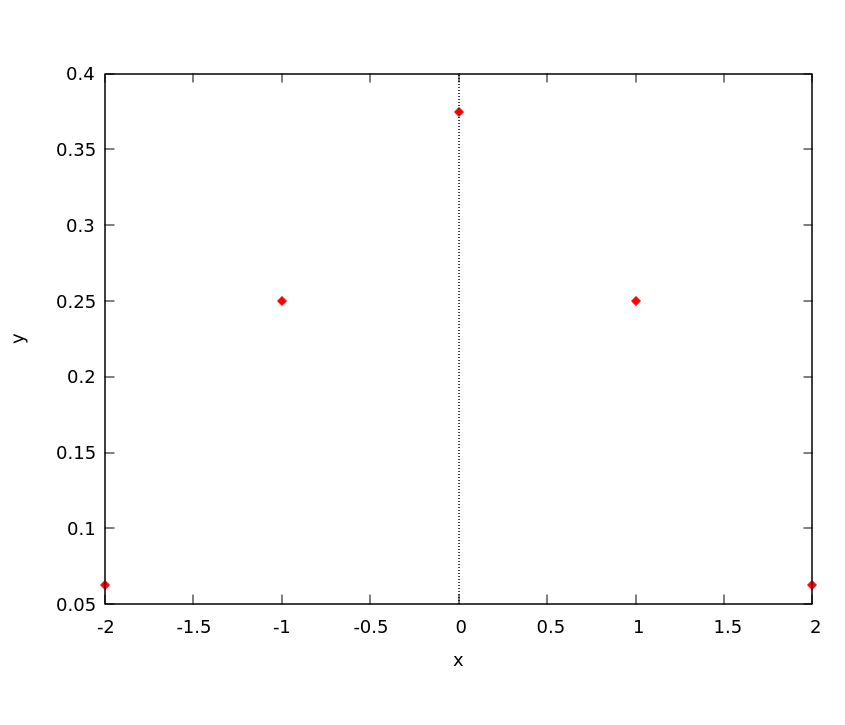
\includegraphics[scale=0.6]{plot}
    \caption{Figure 4.18}
  \end{figure}
  
% BEGIN RECEIVE ORGTBL c
\begin{tabular}{l|l}
\(x\) & \(P(X=x)\)\\
\hline
\(-2\) & \(\frac{1}{16}\)\\
\(-1\) & \(\frac{1}{4}\)\\
\(0\) & \(\frac{3}{8}\)\\
\(1\) & \(\frac{1}{4}\)\\
\(2\) & \(\frac{1}{16}\)\\
\end{tabular}
% END RECEIVE ORGTBL c
\begin{comment}
#+ORGTBL: SEND c orgtbl-to-latex :splice nil :skip 0
| $x$  | $P(X=x)$       |
|------+----------------|
| /    | <              |
| $-2$ | $\frac{1}{16}$ |
| $-1$ | $\frac{1}{4}$  |
| $0$  | $\frac{3}{8}$  |
| $1$  | $\frac{1}{4}$  |
| $2$  | $\frac{1}{16}$ |
\end{comment}
\item [35.]
  \begin{enumerate}[label=(\alph*)]
  \item
    $P(X=1.1) = \frac{{5 \choose 2} + {5 \choose 2}}{{10 \choose 2}} = \frac{4}{9}$.\\
    $P(X=-1)=1-\frac{4}{9}=\frac{5}{9}$.\\
    $E(X)=P(X=-1)\cdot (-1) + P(X=1.1)\cdot 1 = -\frac{1}{15}$
  \item $E(X^2) = 1.1^2 \cdot \frac{4}{9} + (-1)^2\cdot \frac{5}{9} = \frac{9.84}{9}$.\\
    $V(X) = E(X^2) - (E(X))^2 = \frac{49}{45}$
  \end{enumerate}
\item [38.]
  \begin{enumerate}[label=(\alph*)]
  \item
    \begin{equation*}
      \begin{split}
        E(X^2) = 5+1^2 = 6
      \end{split}
    \end{equation*}
    \begin{equation*}
      \begin{split}
        E((2+X)^2)
        &= E(X^2 + 4X + 4) \\
        &= E(X^2) + 4E(X) + 4\\
        &= 6 + 4 + 4\\
        &= 14
      \end{split}
    \end{equation*}
  \item 
    \begin{equation*}
      \begin{split}
        Var(4+3X)
        &= 9Var(X)\\
        &= 9 \cdot 5\\
        &= 45
      \end{split}
    \end{equation*}
  \end{enumerate}
\item [79.]
  $X$ follows hyper-geometric distribution.
  \begin{enumerate}[label=(\alph*)]
  \item
    \begin{equation*}
      P(X=0) = \frac{{6 \choose 0} {94 \choose 10}}{{100 \choose 10}} \approx 0.5223
    \end{equation*}
  \item
    \begin{equation*}
      \begin{split}
        P(X > 2)
        &= 1 - \sum_{i=0}^2\frac{{6 \choose i}{94 \choose 10 - i}}{{100 \choose 10}}\\
        &\approx 0.01255
      \end{split}
    \end{equation*}

  \end{enumerate}
\end{itemize}

\begin{itemize}
\item [5.]
  \begin{proof}
    \begin{equation*}
      \begin{split}
        \sum_{i=1}^n(a_1+\ldots+a_i)P(N=i) &= \sum_{i=1}^na_iP(i \leq
        N \leq n)
      \end{split}
    \end{equation*}
    To go from the first expression to the second expression, we
    simply unwrap the summation and use the distributive law on
    $a_1\ldots a_n$.

    If we take its limit, we get
    \begin{equation*}
      \begin{split}
        \lim_{n\rightarrow \infty}\sum_{i=1}^na_iP(i\leq N \leq n) &=
        \sum_{i=1}^{\infty}a_iP(N \geq i)
      \end{split}
    \end{equation*}
    I don't know how to show this part rigorously, but it's correct
    based on intuition.
  \end{proof}

  \begin{proof}
    Apply the fact we just proved with $a_i=1$ for all $i$.
    \[\sum_{i=1}^{\infty}P(N \geq i) = \sum_{i=1}^{\infty}1 \cdot P(N
      \geq i)= \sum_{i=1}^\infty\underbrace{(1+\ldots+1)}_{i}P(N=i) =
      \sum_{i=1}^niP(N=i) = E(N)\].
  \end{proof}
  \begin{proof}
    Apply it with $a_i = i$ for all $i$, we get
    \begin{equation*}
      \begin{split}
        \sum_{i=1}^\infty i \cdot P(N\geq i)
        &= \sum_{i=1}^\infty (1 + 2 +  \ldots + i) P(N=i)\\
        &= \sum_{i=1}^\infty \frac{(i+1)i}{2} P(N=i)\\
        &= E(\frac{N(N+1)}{2})
      \end{split}
    \end{equation*}
  \end{proof}
\item [7.]
  \begin{proof}
    \begin{equation*}
      \begin{split}
        E(\frac{X-\mu}{\delta})
        &= \frac{1}{\delta}(E(X)-\mu)\\
        &= \frac{1}{\delta}(\mu-\mu)\\
        &= 0
      \end{split}
    \end{equation*}
    \begin{equation*}
      \begin{split}
        Var(Y)
        &= \frac{1}{\delta^2} Var(X)\\
        &= \frac{1}{\delta^2}\delta^2\\
        &= 1
      \end{split}
    \end{equation*}
  \end{proof}
\item [10.]
  \begin{equation*}
    \begin{split}
      E[\frac{1}{X+1}]
      &= \sum_{i=0}^n\frac{1}{i+1}\cdot {n \choose i} p^i(1-p)^{n-i}\\
      &= \frac{(n+1)p}{(n+1)p} \sum_{i=0}^n\frac{1}{i+1}\cdot {n
        \choose i} p^i(1-p)^{n-i}\\
      &= \frac{1}{(n+1)p}\sum_{i=1}^n\frac{1}{i+1} {n \choose i}
      p^{i+1}(1-p)^{n-1}\\
      &= \frac{1}{(n+1)p} \sum_{i=0}^n {n+1 \choose i+1}
      p^{i+1}(1-p)^{n-i}\\
      &= \frac{1}{(n+1)p} \sum_{i=1}^{n+1} {n+1 \choose i} p^i
      (1-p)^{(n+1)-i}\\
      &= \frac{1}{(n+1)p} (\sum_{i=0}^{n+1} {n+1 \choose i} p^i
      (1-p)^{(n+1)-i} - {n+1 \choose 0} p^0(1-p)^{n+1})\\
      &= \frac{1}{(n+1)p}((p+1-p)^{n+1}-(1-p)^{n+1})\\
      &= \frac{1-(1-p)^{n+1}}{(n+1)p}
    \end{split}
  \end{equation*}
\item [19.]
  Running out of time. See handwritten version on the last few pages.
\end{itemize}


\end{document}
